Actuators are an important part of any control system because they are the ones responsible for bringing it to the desired state. They do this by applying forces on the system. In our case, the actuators are the motor and the propellers. Figure x displays the actuators' configuration. Ardupilot, which is the ''brain'' of our control system and has the controller implemented on it is connected to the speed controller, which is in charge of controlling the motor through a PWM signal. 

\begin{figure}[H]
  \centering
    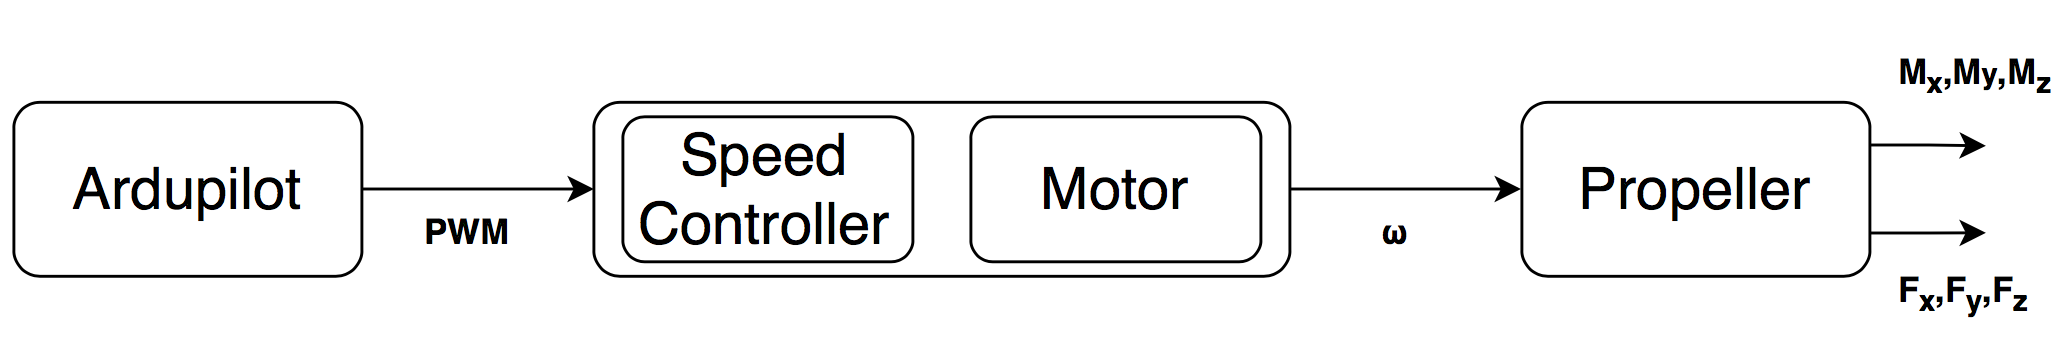
\includegraphics[width=1\textwidth]{images/ablockd.png}
	\caption{Actuators Block Diagram.}
	\label{ablockd}
\end{figure}

Each motor produces an angular velocity $\omega$, therefore the propeller spins at that defined angular velocity. In this chapter, we will be introducing more comprehensible models for both motor and propeller as well as some experiments regarding the PWM signal - motor speed relationship.

\section{Propeller model}
For this part of the report, we have decided not to take into account the aerodynamic forces that act on the propeller, therefore neglecting the air friction, the flapping of the biased and the ground effect. This enables us to create a simpler model, which is easy to understand and implement.

The thrust $F_{i}$ and the moment across the $M_{i}$ along the $u_{z}$ axis can be written as functions of angular velocities such as:

\begin{equation}
	F_{i}=K_{T}\omega_{i}^{2}
\end{equation}

\begin{equation}
	M_{i}=K_{M}\omega_{i}^{2}
\end{equation}

where the constant related to thrust $K_{T}$ and the constant related to the moment $K_{M}$ can be describes as:

\begin{equation}
	K_{T}=c_{T}\frac{\rho D^{4}}{4\Pi^{2}}
\end{equation}

\begin{equation}
	K_{M}=c_{P}\frac{\rho D^{5}}{8\Pi^{2}}
\end{equation}

with D= being the diameter of the propeller, $\rho$ being the air density, $ c_{T} $ and $ c_{P} $ being the thrust and power coefficient. We are considering these values to have small values (<0.2) based on what we have read from other projects.

Therefore:

\begin{equation}
	K_{T}\approx 1.45\times10^{-5}
\end{equation}

\begin{equation}
	K_{M} \approx 3.5\times10^{-7}
\end{equation}

%reference

We can write $K \approx K_{M}/K_{T}=4.1\times10^{-7}=0.024$. The forces and moments can now be expressed as:

\begin{equation}
\label{motor1} 
	F_{i}=K_{T}\omega_{i}^{2}
\end{equation}

\begin{equation}
\label{motor2} 
	M_{x}=(\omega_{2}^{2}-\omega_{4}^{2})K_{T}D=(F_{2}-F_{4})D
\end{equation}

\begin{equation}
\label{motor3} 
	M_{y}=(\omega_{1}^{2}-\omega_{3}^{2})K_{T}D=(F_{1}-F_{3})D
\end{equation}

\begin{equation}
\label{motor4} 
	M_{z}=(\omega_{1}^{2}+\omega_{3}^{2}-\omega_{2}^{2}-\omega_{4}^{2})K_{M}=(F_{1}+F_{3}-F_{2}-F_{4})K
\end{equation}

where D is expressed in centimetres.

\section{Motor model}
Providing a signal to the motor is done through Ardupilot, using PWM, which enables providing an analogue signal by digital means.  In order to create a PWM signal, we have used the \textit{write.Microseconds()} function from the\textit{Servo.h} library within the Arduino IDE environment. The role of the speed controllers is to turn the PWM signal into a three-phase signal to feed the BLDC motors.

Each motor receives a three-phase signal that is proportional with the angular velocity $\omega$. In general, the behaviour of a motor can be analysed by looking at the electrical and mechanical part of its structure. These parts are represented in Figure \ref{dc}. 

\begin{figure}[H]
  \centering
    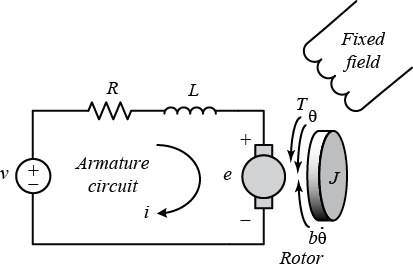
\includegraphics[width=0.6\textwidth]{images/dc.png}
	\caption{Electrical and Mechanical part of the motor.\cite{MotorFig}}
	\label{dc}
\end{figure}

A second order system can be obtained by writing the equations that describe the electrical and mechanical part as:

\begin{equation}
	V=RI+L\frac{dI}{dt}+K_{e}\dot{\theta}
\end{equation}

\begin{equation}
   K_{e}I = J \ddot{\theta}+b\dot{\theta}
\end{equation}

The transfer function can be taking the Laplace transform of each equation and manipulating it into:

\begin{equation}
\label{modelm} 
   \frac{\omega}{PWM}=\frac{K_{e}}{(Js+b)(Ls+R)+K_{e}^{2}}
\end{equation}

where $\omega$ is the angular velocity of the motor, PWM is the signal to the motor, $K_{e}$ is the electromotive constant, J is the rotor's moment of inertia, b is the damping ratio of the mechanical system, L is the inductance, R is the resistance and I is the measurement of the current.

Equation \ref{modelm} can be further simplified and written as a first order system, since it is difficult to measure all the motor parameters:\cite{Report1}

\begin{equation}
   \frac{\omega}{PWM}=\frac{k_{i}}{\tau s+1}
\end{equation}

where $\tau$ is the time constant of the system and $k_{i}$ is the DC gain. 

\section{Electronic Speed Controllers}
ESCs have 5 input pins, 3 of which come from the flight controller. These 3 wires supply the signal for the ESC to translate into the angle of the shaft for the motor. Before ESCs can be used, they need to be properly calibrated. Programming additional settings is optional, but in most cases necessary too. Normally, the calibration for UAVs is done by setting the throttle to full on the radio controller before powering the ESCs. However, since the board translates the throttle signal into a PWM signal, it is possible to calibrate and run the motors directly from the flight controller by sending a PWM signal using software.

\subsection{Calibration and Programming}
The calibration is done by first sending the maximum length of signal the user wishes to use. The ESC emits sounds that are brand-specific and indicate whether the signal was successfully recognised or not. Once the maximum signal is accepted, the user the emits the minimum signal and waits for approval. Additional sound is then emitted, indicating that the calibration was successful.

Using Arduino's Servo library, a self-explanatory built-in function \textit{servo.writeMicroseconds(int value)} is used to send the signal. By default, the library has the minimum signal set to 544$\mu s$ and the maximum - to 2400$\mu s$. For this project, we shortened the range down to 700$\mu s$ and 2000$\mu s$ for both signals respectively. A commented code used to calibrate the ESC connected to the first pin of the board can be seen in Listing \ref{code:calib}.

\lstinputlisting[language=C++, caption={Calibrating the ESC.}, label={code:calib}]{Arduino/ESCCalib/ESCCalib.ino}

Programming additional settings of the ESC is done in a similar manner - by sending minimum and maximum signals after the ESC emits particular sounds, indicating wanted selections. The programmable features and selections are brand-specific and can be found in the datasheets. For the purposes of this project, the ESCs have been programmed to include two features - brake mode off and selection of li-ion battery.

\section{Ardupilot and Motor Identification}
This section will show the experiments that we have carried out in regards to the motor as well as Ardupilot frequency analysis.

\subsection{APM Frequency}
Due to lack of proper documentation, it was necessary to measure the frequency of the signals sent out by the flight controller. To do so, an oscilloscope was connected to one of the output pins of the board. Then, using the servo library, a signal was sent out. The interval between signals was found to be 20$ms$, therefore, the frequency of the board is 50$Hz$, as seen in Figure \ref{oscillo1}.
\begin{figure}[H]
  \centering
    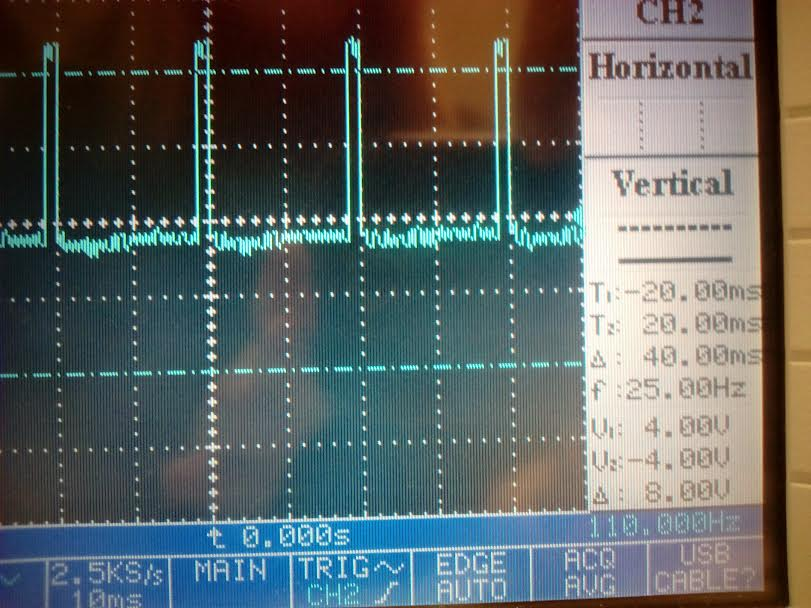
\includegraphics[width=0.5\textwidth]{images/oscillo1.jpg}
	\caption{Oscilloscope Measuring APM's Frequency.}
	\label{oscillo1}
\end{figure}

The second experiment on the board was then made to determine how the flight controller handles the output signals during those 20$ms$. First two outputs of the APM were connected to the oscilloscope, both utilizing the Servo library to send signals of length of 2000$\mu s$. Results can be seen in Figure \ref{oscillo2}.
\begin{figure}[H]
  \centering
    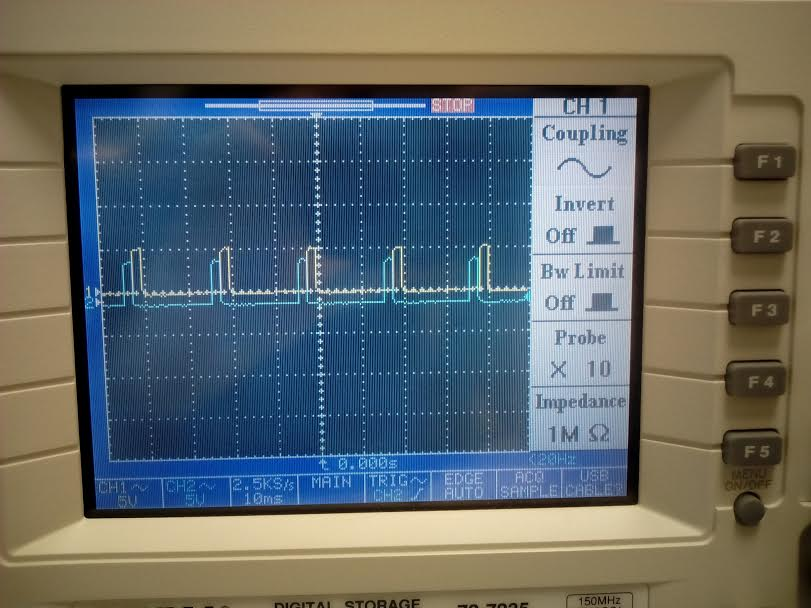
\includegraphics[width=0.5\textwidth]{images/oscillo2.jpg}
	\caption{Readings of the Two Output Signals.}
	\label{oscillo2}
\end{figure}

Then, for further testing purposes, both outputs were given different values in two scenarios, as seen in Figure \ref{oscillo3}.

\begin{figure}[H]
  \centering
    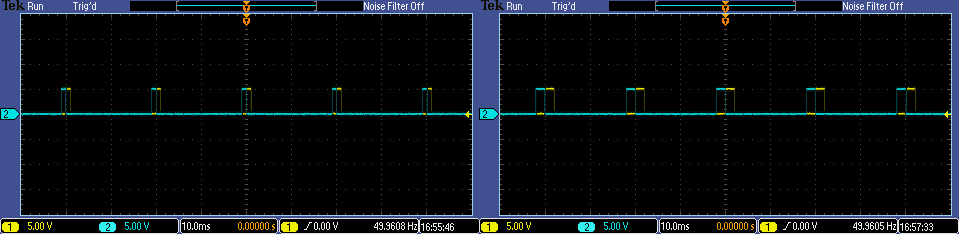
\includegraphics[width=0.5\textwidth]{images/oscillo3.png}
	\caption{Left - Signals Running at 2000$\mu s$; Right - 700$\mu s$.}
	\label{oscillo3}
\end{figure}

From this, two conclusions can be made:
\begin{enumerate}
\item If the first signal is shorter than the second one, the second signal will still follow right after the first signal ends. In other words, the APM leaves no gaps between the outputs.
\item Since the board runs at the frequency of 50$Hz$ and has a period of 20$ms$, this leaves $\frac{20}{8} = 2.5ms$ maximum length for each output signal. The servo library is hard-capped at 2.4$ms$ and thus is well within the limits of the board.
\end{enumerate}

\subsection{Expected and Real Motor Performance}
The motors used in the prototype specify to be rated at $K_v$ of 980. $K_v$ is a constant describing the ratio between RPM and the applied voltage and is expressed as $K_v = \frac{RPM}{V}$. Derived from this, voltage's effect on the RPM can be seen in Figure \ref{KvPlot}.
\begin{figure}[H]
  \centering
    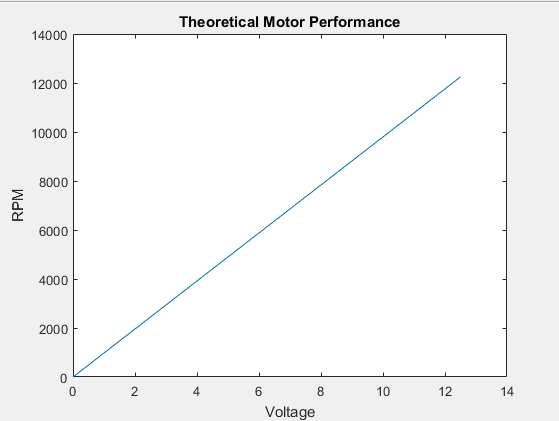
\includegraphics[width=0.8\textwidth]{images/KvPlot.png}
	\caption{Expected Motor Performance.}
	\label{KvPlot}
\end{figure}
With a fully charged battery, the RPM is expected to be $980\times 12.6V = 12348 RPM$.
In order to confirm this, the actual RPM was measured using SHIMPO DT-205 digital tachometer. A piece of reflective paper was taped to one of the motors so that the tachometer would have something to lock onto, as seen in Figure \ref{tachometer}.

\begin{figure}[H]
  \centering
    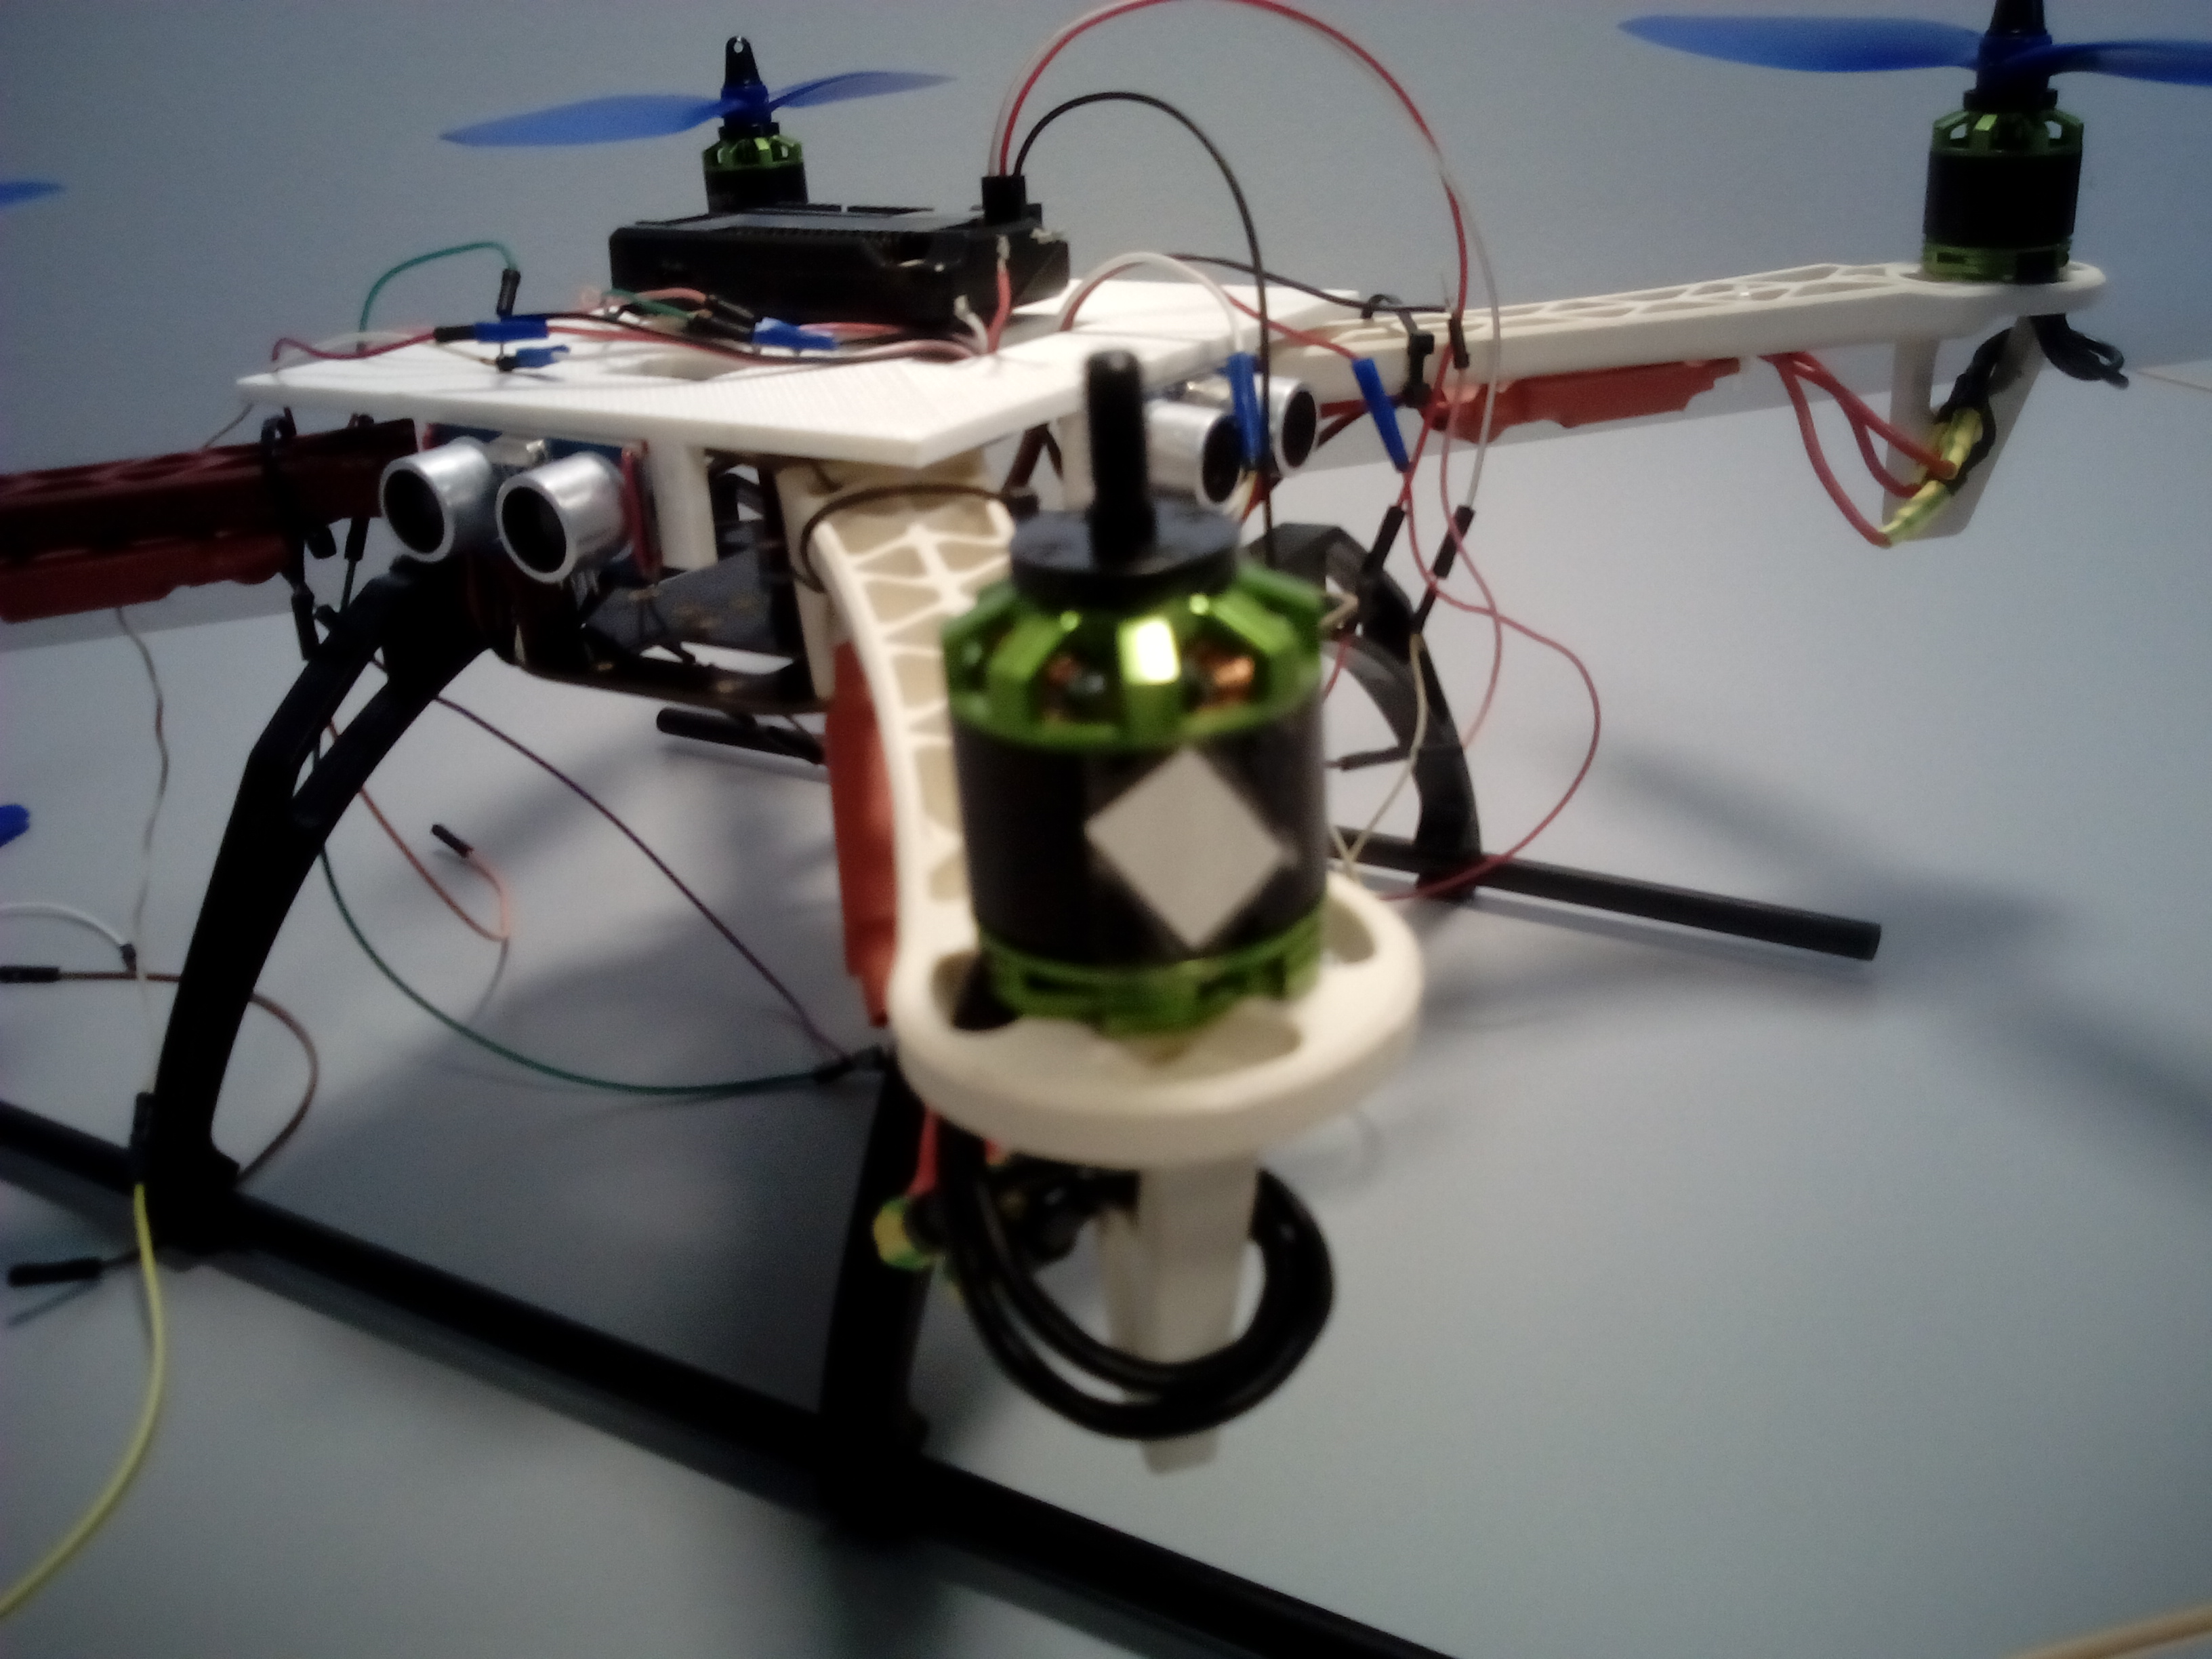
\includegraphics[width=0.5\textwidth]{images/tachometer.jpg}
	\caption{Reflective Paper on the Motor.}
	\label{tachometer}
\end{figure}

While it is possible that the mounted propeller could affect the speed of the motor, the measurements had to be done with no propeller on the motor, as it would not only make it difficult to detect the reflective paper, but also be dangerous, since the thrust generated by the fully operational motor is unknown.
By sending the maximum signal from the board, the RPM was measured to be 11468, with a small possible error. The measured number does not match the $K_v$ given in the datasheet and there are many possible causes. However, it the result is not too far off the expected value, so the there are no major problems.

\subsection{Measuring Motor Speed}
In order to use the board's output signal as an input in a mathematical model, it is necessary to find an equation to translate it into an angular rate.
First, an equation has been found that describes the relationship between motor's RPM, ESC's output signal frequency and number of motor poles \cite{RPMEq}:

\begin{equation}
\label{voltage1}
	RPM = \frac{120\times f}{n}
\end{equation}
Here, $f$ is the frequency and $n$ is the number of poles (in the case of this project - 14).

Therefore, it is possible to measure the frequency at various output values, which can then be used to define an equation that uses the board's signal length as an input value and results in an RPM.

The frequency was measured using an (NAME) oscilloscope and by connecting the probe's ground clip to the ground of the battery and the probe tip to any one of the wires between motor and the ESC. Then, by providing different output signals in some arbitrary range from the flight controller, the frequency was measured on the oscilloscope screen. An on-board filter was used to filter out some noise, especially at lower output signals. The recorded frequency was later converted into RPM using Equation \ref{voltage1}, for later comparison. The output signal lengths and the corresponding frequencies converted into RPM can be seen in Table \ref{FreqTable}.

While measuring, it was observed that the frequency would never reach stable readings and therefore, a sizeable error is possible between measurements. Because of that, RPM was manually measured using the tachometer at same output values, as seen in Table \ref{RPMTable}.

While measuring with tachometer, the error appeared to be less significant.
The two Tables \ref{RPMTable} and \ref{FreqTable} were then plotted to see the difference, which is seen in Figure \ref{RPMvsFreq}.

\begin{figure}[H]
  \centering
    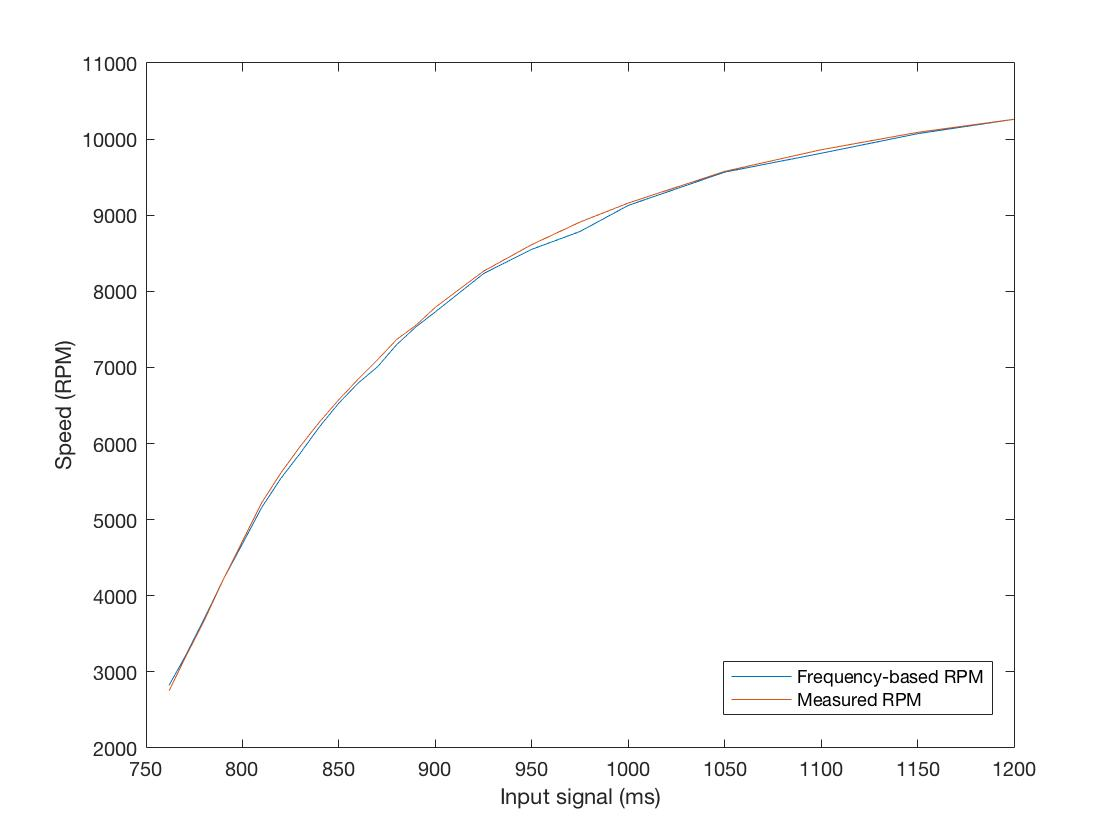
\includegraphics[width=1\textwidth]{images/rpm66.jpg}
	\caption{Plotted Values of Manually Measured and Frequency-based RPM.}
	\label{RPMvsFreq}
\end{figure}

The graphs show some difference between the two measuring methods. The frequency method gives more or less linearly downscaled values. Due to lack of accurate way of determining which readings are correct, it was chosen to go with the tachometer measurements. The process of obtaining measurements with an oscilloscope took more time and was, therefore, deemed inefficient.

In order to make use of these findings, the RPM values have to be converted into $rad/s$ for use as angular rate. The conversion equation is:
\begin{equation}
\label{RPMConvert}
	\omega = \frac{2\pi \times RPM}{60}
\end{equation}

\subsection{Measuring Speed in Desired Range}
Once it was decided how to measure angular velocity, an output range of 1500 to 2400 $\mu s$ was chosen. The RPM was measured at certain microseconds signal, with increments of 100 across all four motors and converted into $rad/s$. The measured values have been put into Table \ref{speedTable}.
The plots of the angular velocity (see Figure \ref{radsPlots}) have revealed interesting discoveries - all four motors run at different speeds. Moreover, there seems to be no linear relationship between them throughout the whole range, so it is impossible to express one motor's speed as a function of another motor multiplied by some constant. After failing to find the cause of the difference in the speeds, a conclusion was reached that the motors run at different speeds due to their structure and therefore cannot be changed.

\begin{figure}[H]
  \centering
    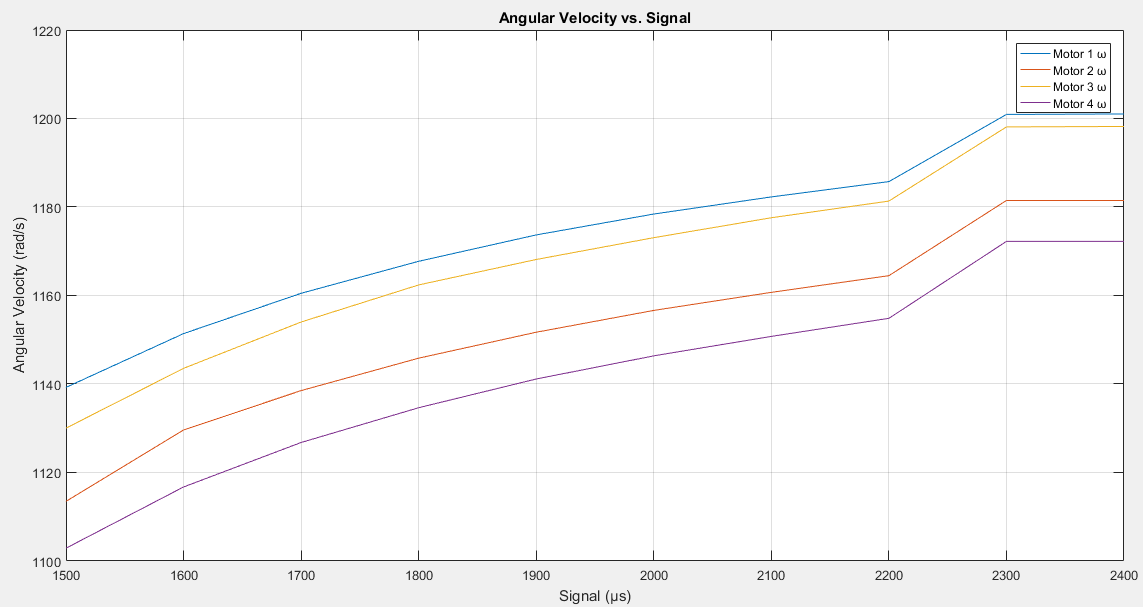
\includegraphics[width=1\textwidth]{images/radsPlots.png}
	\caption{Angular Velocity vs. Output Signal for all Motors.}
	\label{radsPlots}
\end{figure}

In order to use this data, it was decided to first reduce the range of the measurements - from 1500 to 2000 $\mu s$. Then, utilising the $polyfit$ function in Matlab, it is possible to derive linear equations with signal as input and angular velocity as output. The equations have been plotted in Figure \ref{RadsTrendline}.

\begin{figure}[H]
  \centering
    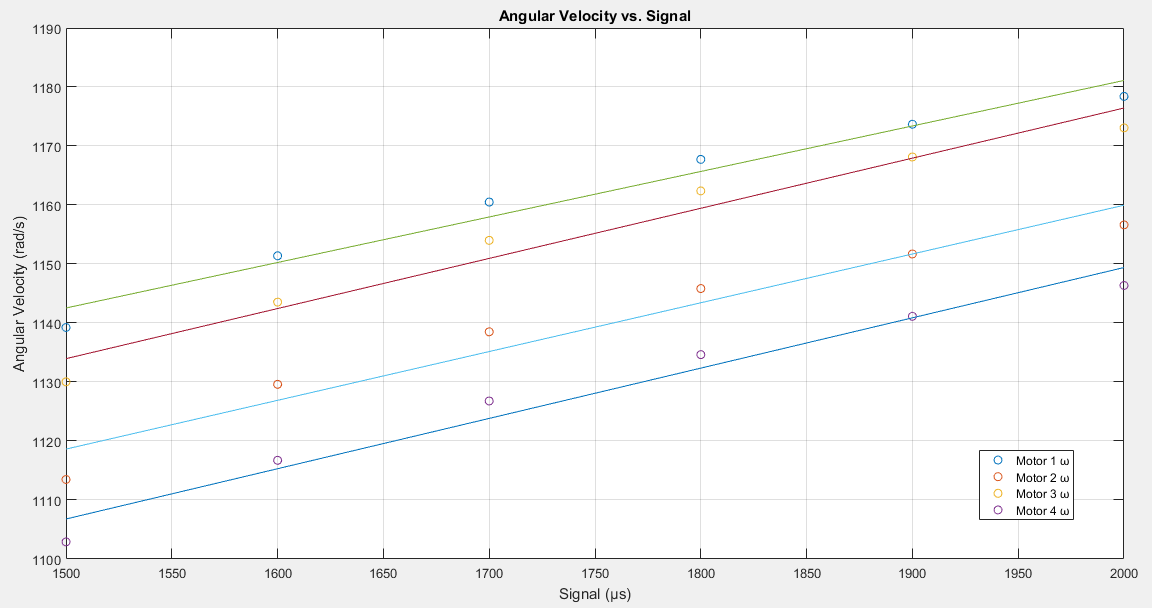
\includegraphics[width=1\textwidth]{images/polyfits.png}
	\caption{Linear Relationship between Signals and Angular Velocities.}
	\label{RadsTrendline}
\end{figure}
The following equations for the linear functions then are:
\begin{center}
\begin{equation}
	\omega _1 = 0.0771\times PWM1 + 1026.837
\end{equation}



\begin{equation}
	\omega _2 = 0.0826\times PWM2 + 994.62
\end{equation}



\begin{equation}
	\omega _3 = 0.0849\times PWM3 + 1006.507
\end{equation}



\begin{equation}
	\omega _4 = 0.0852\times PWM4 + 978.91
\end{equation}
\end{center}
The linear equations do not fit the original graph perfectly, but require less computational power to perform calculations. It is possible to instead acquire $2^{nd}$ polynomial that would be a more accurate estimation of the original graph, however, that would require more time to compute. This question will be briefly addressed in the discussion chapter. 

\subsection{Operating Range}
Due to lack of linearities in the equations expressing the angular velocity, some operating range has to be defined when calculating coefficients, to find reasonable approximates that would hold true for the most of the prototype's function. Given the drone's main objective - hovering - it is not a far-fetched idea to chose operating point as $TWR = 1$. A newtonmeter was attached to the first motor, with the propeller mounted on it. Then, a signal from the board was sent to the motor, starting at 700 and increasing by 100, up to 2400 $\mu s$. The recorded data had significant amount of noise and had to be filtered out in Matlab. Figure \ref{forcePlot} shows the measured force in newtons, where every significant increase in the force shows increment in the signal.
\begin{figure}[H]
  \centering
    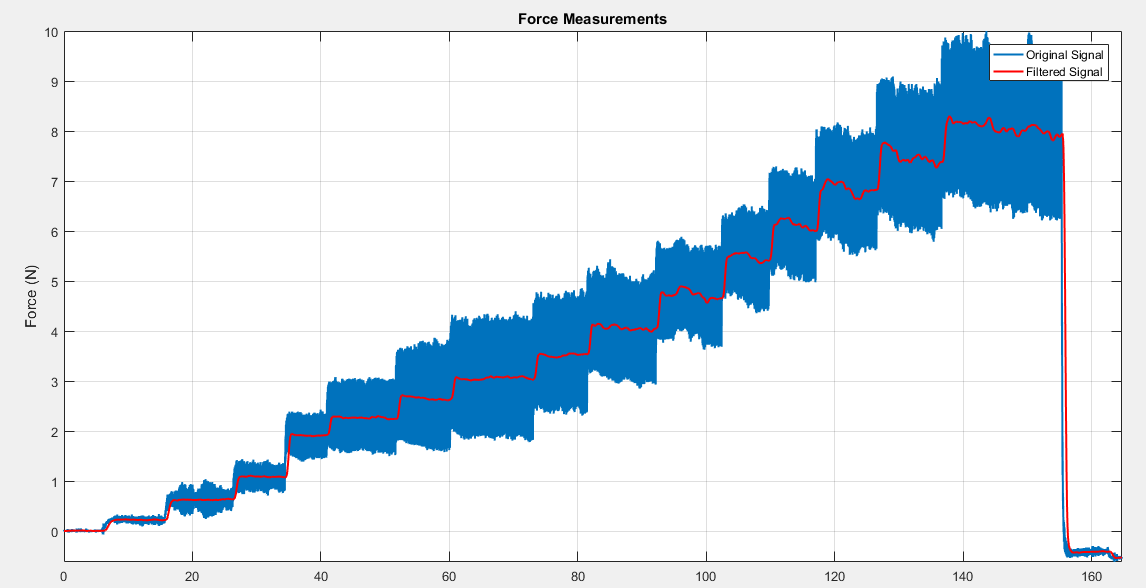
\includegraphics[width=1\textwidth]{images/forceMeasurements.png}
	\caption{Thrust Force Created by First Motor.}
	\label{forcePlot}
\end{figure}
The test reveals two things: at maximum speed, the motor can provide solid $8N$ thrust and at higher signals coming in from the board, some overshoot in the motors can be seen, which, in later steps, will have to be taken into consideration.

Given the fact that the drone is drawn to the ground by a $14N$ force, each motor needs to produce about $\frac{14N}{4} = 3.5N$ thrust. Looking at the plot of the test in Figure \ref{forcePlot}, first motor reaches this point at 1499$\mu s$ signal coming from the APM, which, based on Figure \ref{radsPlots}, is equal to 1139$rad/s$. Then, using same graphs, it is possible to find the input signals corresponding to same angular velocity for the remaining motors. These values will be given in Table \ref{motorCoeffs}.
The coefficients and performance of the motors will be centred around these values.

\subsection{Measuring Motor Coefficients}
First, through trial and error, the deadzones for when the motors are receiving a signal from the flight controller but are not spinning yet were found (see Table \ref{motorCoeffs}).

The motor time constant $\tau$ is described as the time it takes the motor to reach 63\% of its expected speed, since the receiving the signal. To do this, PASPORT Rotary Motion Sensor PS-2120A has been connected to one of the motors. Then, using the SPARKvue software, the angular velocity of the motor for a specific time frame was obtained. A signal was sent from the flight controller to the motor and the angular velocity was plotted against the time, as seen in Figure \ref{timeconstant}.

\begin{figure}[H]
  \centering
    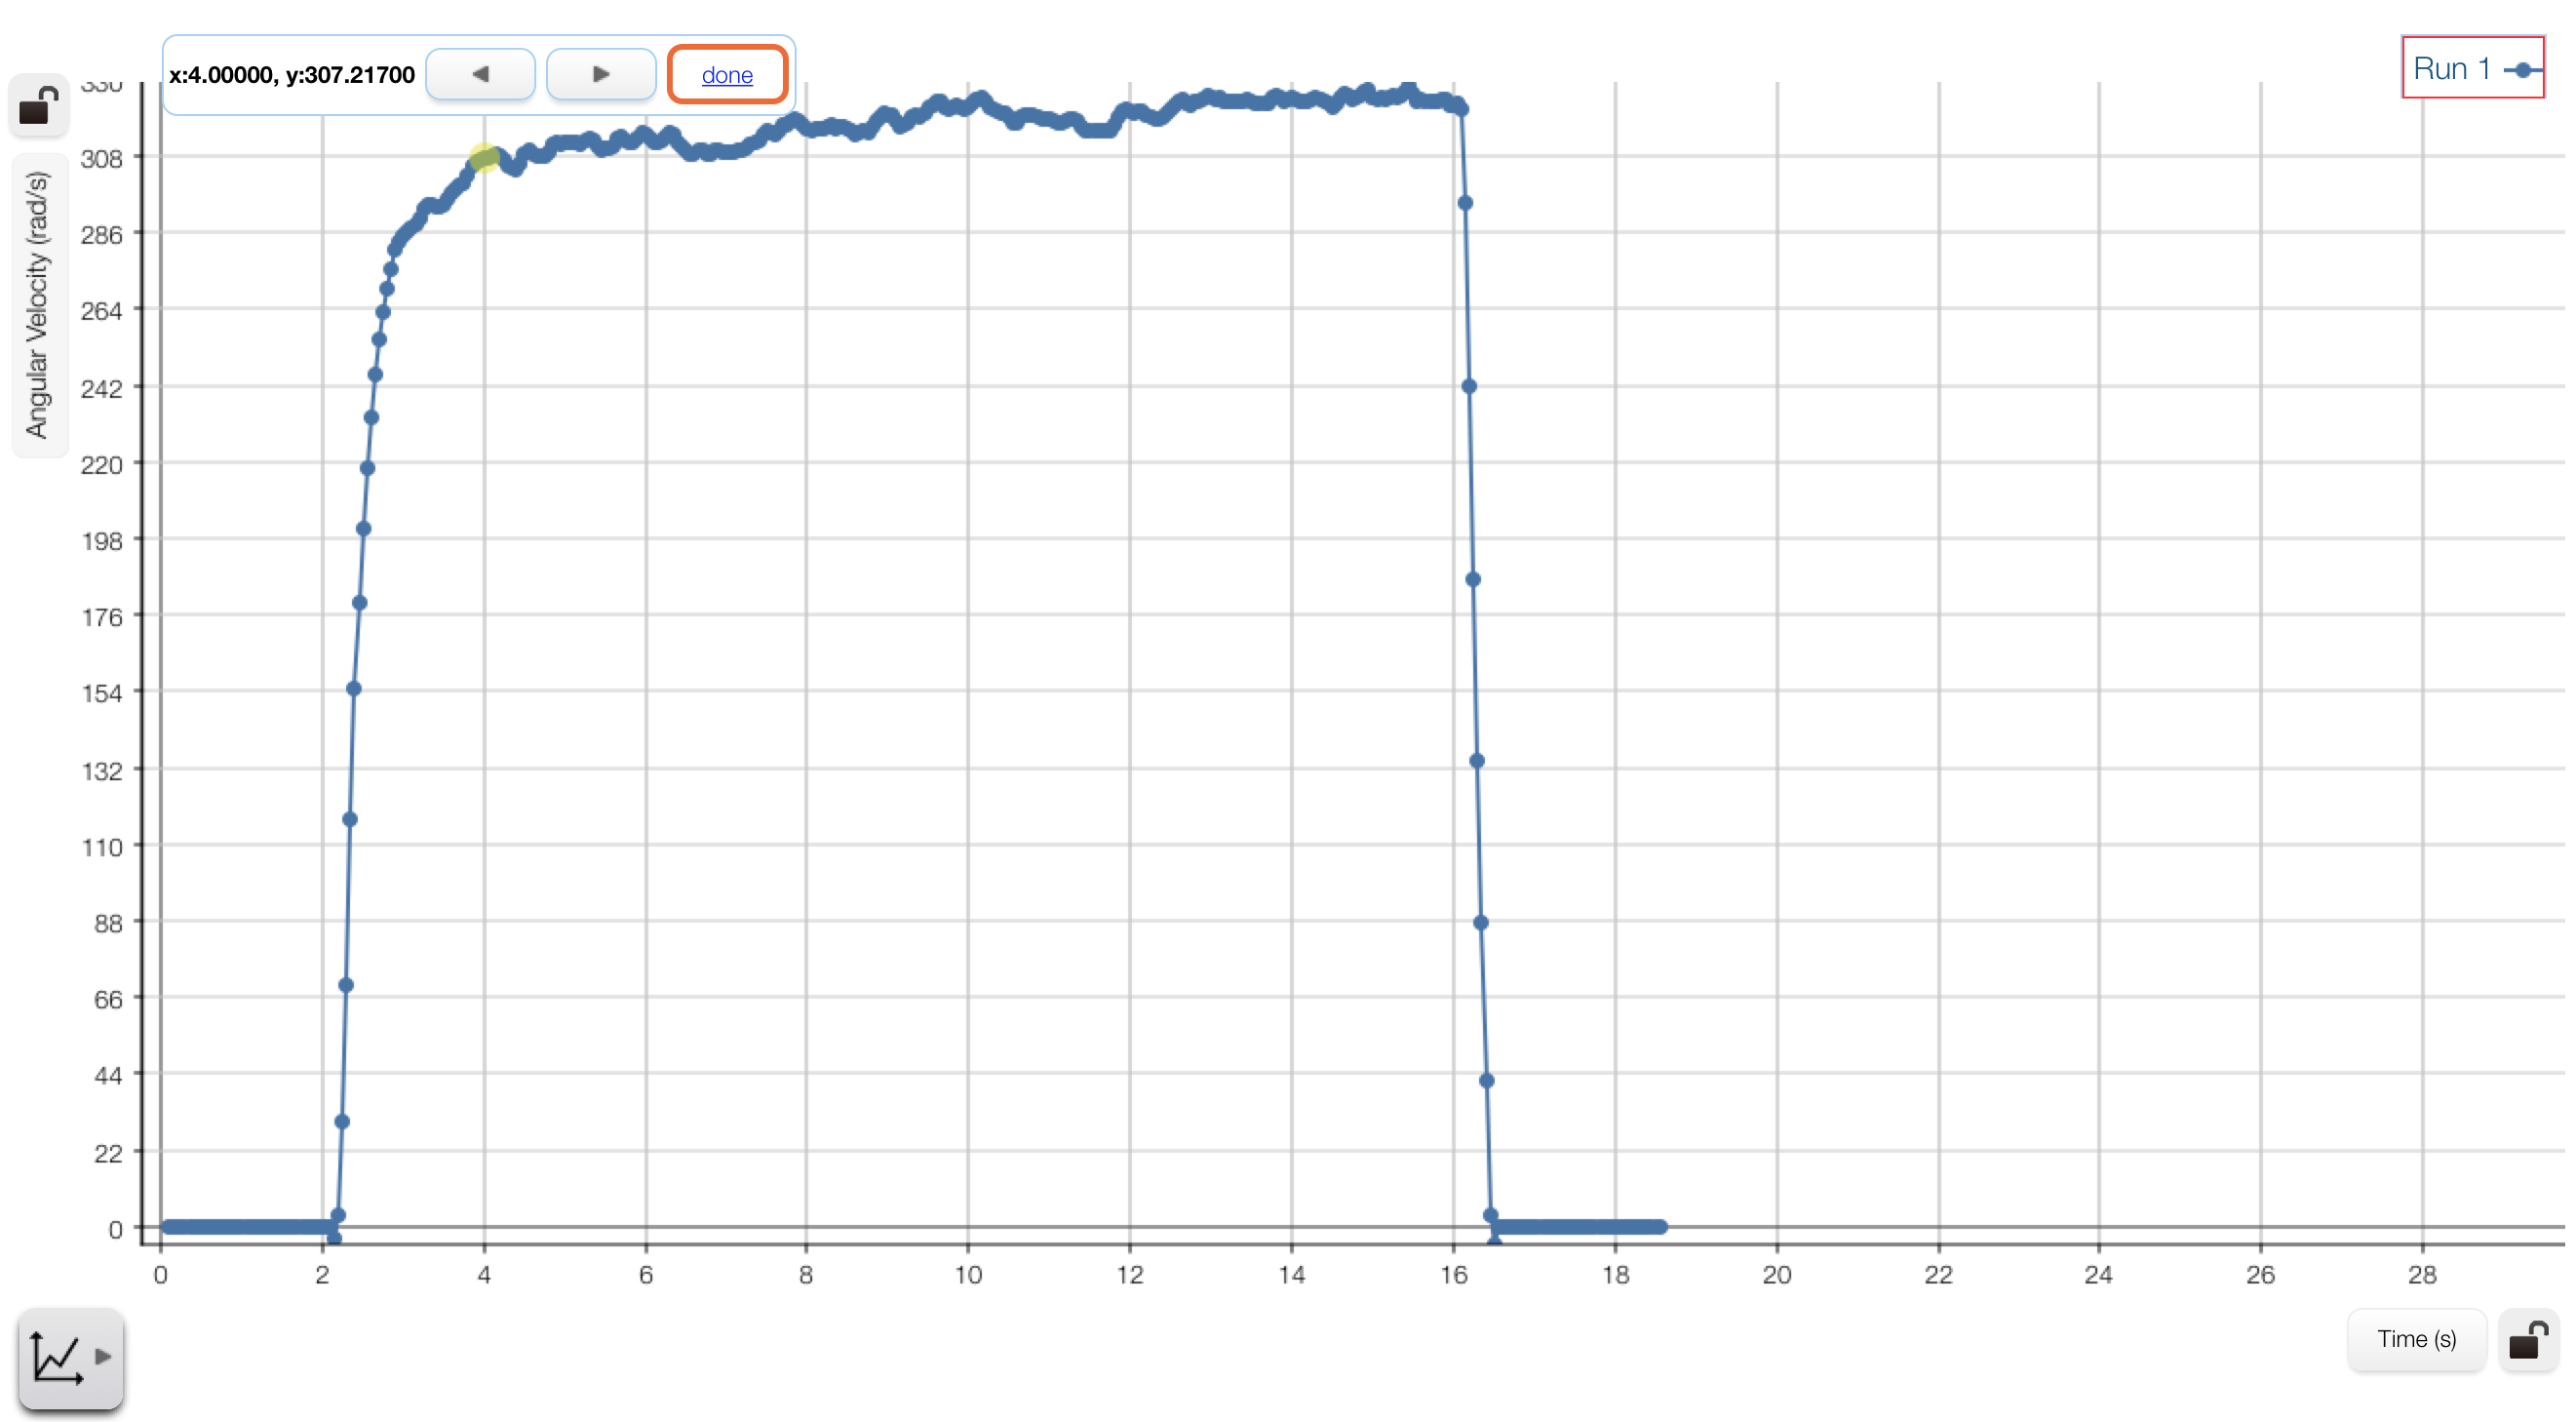
\includegraphics[width=0.8\textwidth]{images/timeconstant.png}
	\caption{Angular Velocity vs. Time.}
	\label{timeconstant}
\end{figure}

The readings were a bit distorted due to the placement of rotary sensor - the rubber band connecting the motor and the sensor's wheel was not in a fixed position, slowing down the motor at times. Nevertheless, the important part was the rise of the angular velocity. It was determined that 63\% of the peak value 308$rad/s$ was reached in $0.361s$.

The DC gain $k_i$ is the constant, describing the relationship between angular velocity $\omega$ and the $PWM$ input signal. An equation for a specific motor's angular velocity can be given as:
\begin{equation}
\label{kieq}
	\omega = k_i*(PWM - PWM^{Dz})
\end{equation}

where $PWM^{Dz}$ is the deadzone of the motor.
Since the deadzone for all motors is known and so is the angular velocity and the $PWM$ signal at a specific point, it is then possible to use Equation \ref{kieq} to find $k_i$ for the motors. The full list of coefficients is given in Table \ref{motorCoeffs}.

\begin{table}[H]
\centering
\begin{tabular}{|c|c|c|c|}
\hline
Motor	& $k_i$ 	& $PWM$ 	& $PWM^{Dz}$ 	\\ \hline
1 		& 1.585104	& 1499		& 780			\\ \hline
2 		& 1.22626	& 1710		& 780			\\ \hline
3 		& 1.465694	& 1559		& 781			\\ \hline
4 		& 1.058975	& 1857		& 781			\\ \hline

\end{tabular}
\caption{Motor Deadzones, $k_i$ Coefficient and the Lift-off $PWM$ Requirements.}
\label{motorCoeffs}
\end{table}

The transfer function with the coefficients in place has been modelled in Simulink, as seen in Figure \ref{motorSimulink}.
\begin{figure}[H]
  \centering
    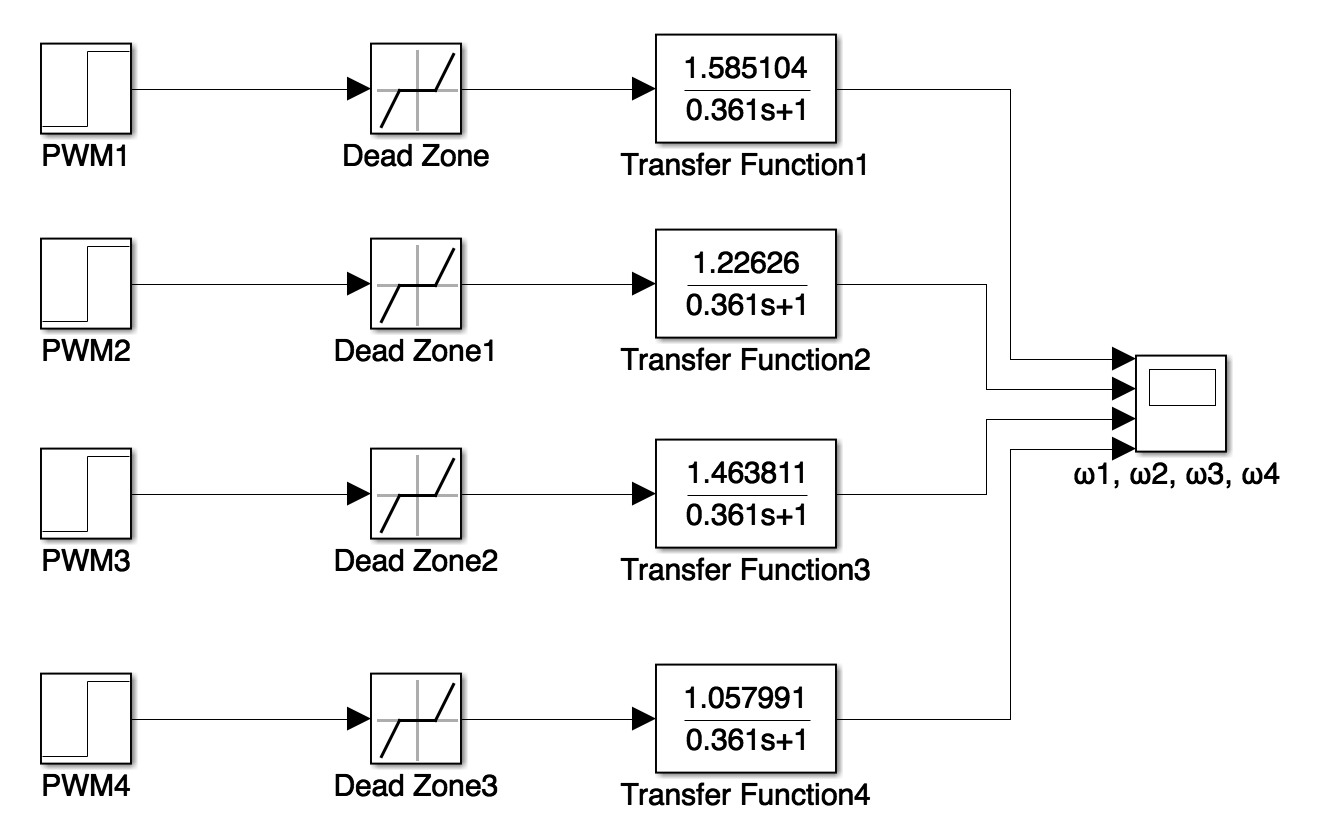
\includegraphics[width=0.8\textwidth]{images/simulinkmotor.png}
	\caption{Simulink Model of the Motors.}
	\label{motorSimulink}
\end{figure}

By giving the PWM values from Table \ref{motorCoeffs}, the simulation shows angular velocity of all four motors. It can be seen in Figure \ref{motorScope} that the speeds still do not match perfectly. This is because none of the functions are linear, giving only the approximations of the coefficients used in the model and not exact values. As such, some controller will need to be implemented to try and compensate for the differences.

\begin{figure}[H]
  \centering
    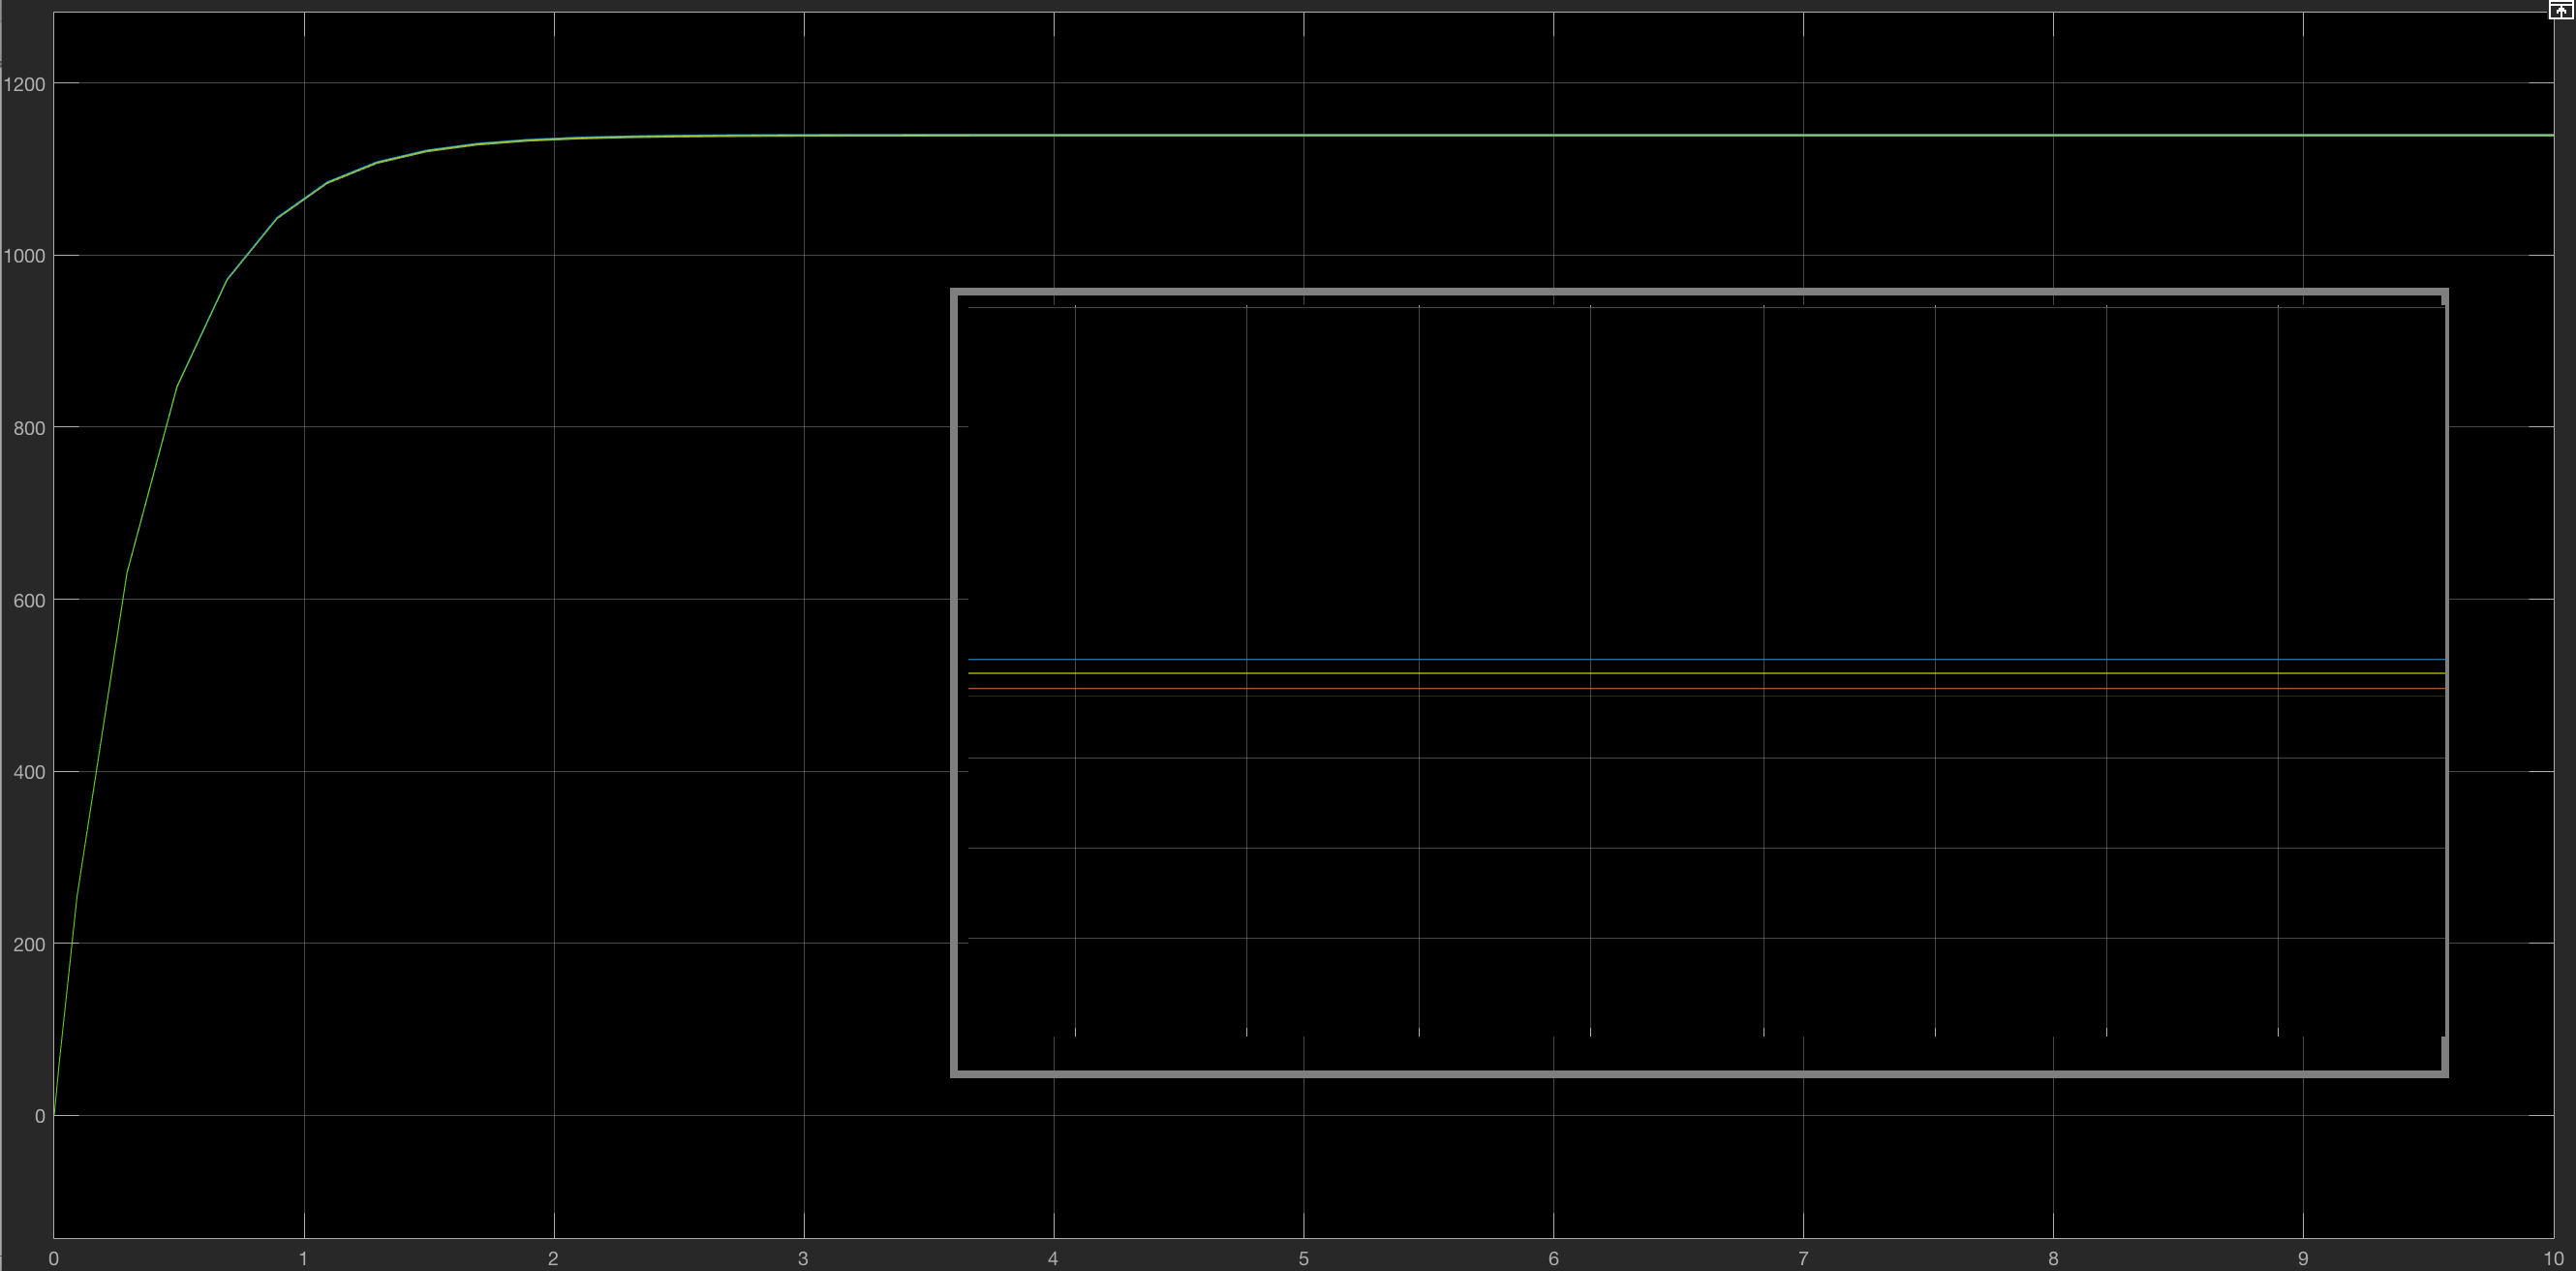
\includegraphics[width=1\textwidth]{images/scopewithcloseup.png}
	\caption{The Output of the Model and a Close Up.}
	\label{motorScope}
\end{figure}